Formula y evalúa $\iiint_E z\,dV$ para el sólido representado en la figura.

\begingroup
\shorthandoff{>}
\begin{center}
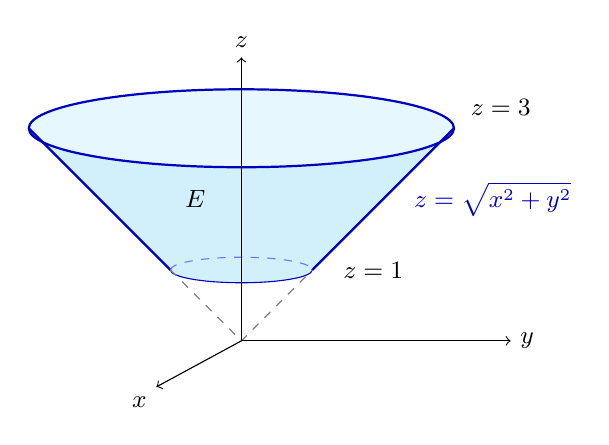
\begin{tikzpicture}[every node/.style={font=\small},scale=.9]
    \fill[cyan!18] (-1,1) -- (-3,3)
        arc[start angle=180,end angle=360,x radius=3,y radius=.55]
        -- (1,1) arc[start angle=0,end angle=-180,x radius=1,y radius=.18] -- cycle;
    \fill[cyan!10] (0,3) ellipse (3 and .55);
    \draw[blue!75!black,thick] (-1,1) -- (-3,3) (1,1) -- (3,3);
    \draw[blue!75!black,thick] (0,3) ellipse (3 and .55);
    \draw[dashed,blue!55] (-1,1) arc[start angle=180,end angle=0,x radius=1,y radius=.18];
    \draw[blue!75!black] (-1,1) arc[start angle=180,end angle=360,x radius=1,y radius=.18];
    \draw[dashed,gray] (-1,1) -- (0,0) -- (1,1);
    \draw[->] (0,0) -- (3.8,0) node[right] {$y$};
    \draw[->] (0,0) -- (-1.2,-.65) node[below left] {$x$};
    \draw[->] (0,0) -- (0,4) node[above] {$z$};
    \node[right] at (3.1,3.3) {$z=3$};
    \node[right] at (1.3,1) {$z=1$};
    \node[right,blue!75!black] at (2.3,2) {$z=\sqrt{x^2+y^2}$};
    \node at (-.65,2) {$E$};
\end{tikzpicture}
\end{center}
\endgroup
